\subsection{Architekturentscheide}
Wesentliche Entscheide, welche wir während dem Projekt getroffen haben, sind hier detailliert begründet. Auch Gedanken oder Ideen, welche wir während der Analysephase hatten, dann aber verworfen haben, sind hier aufgeschrieben.

\subsubsection{Domain-Design-Entscheid}
Schon sehr für im Projekt kam die Idee auf, die BrainstormingFindings in verschiedene Arten (z.B. GeneralFinding oder SoftwareFinding) zu unterteilen. Damit wollten wir erreichen, dass nicht jeder Ideentyp für jedes BrainstormingFinding zur Verfügung steht, zumal es auch nicht unbedingt für jede Kombination Sinn ergibt, diesen Ideentypen dafür anzubieten. Zum Beispiel ergibt es wenig Sinn die PatternIdea bei einem GeneralFinding anzubieten. Dies würde eher bei einem SoftwareFinding zum Einsatz kommen.

\begin{figure}[h]
	\centering
	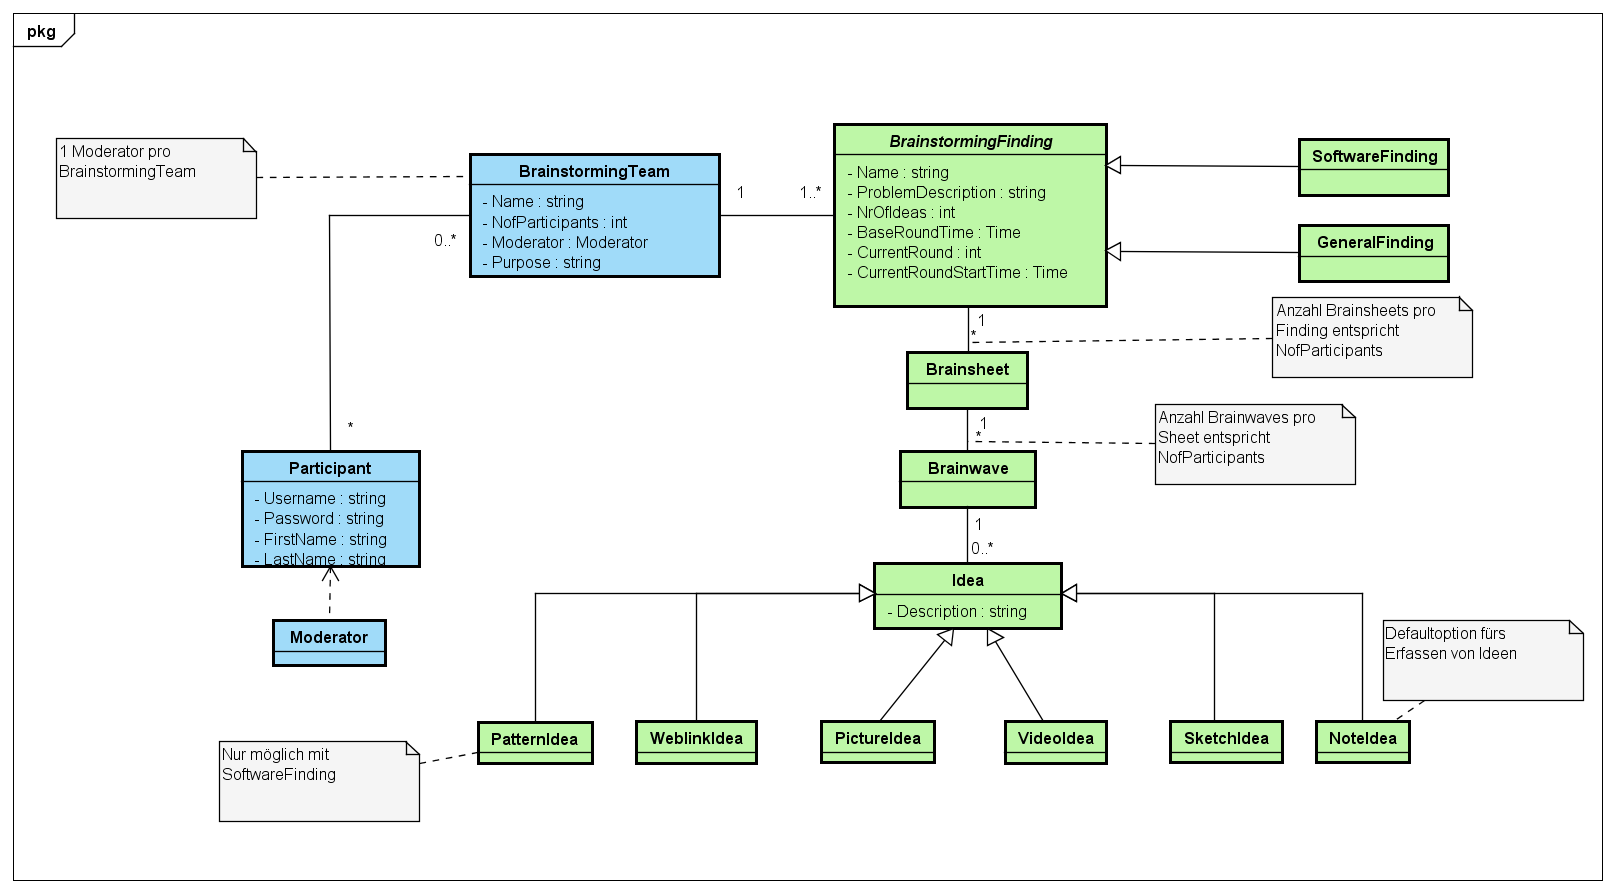
\includegraphics[width=1\linewidth]{img/domain-analyse/DomainModell-Methode635-Entwurf}
	\caption{Erster Entwurf vom Domain Modell BrainingOutOfBox}
	\label{fig:domainmodell-methode635-entwurf}
\end{figure}

Doch dabei kommt die Überlegung auf, was wenn es noch andere Patterns als nur Software-Patterns gibt, welche man zur Verfügung stellen will. Dann müssten noch mehr solcher logischen Zusammenhänge beachtet werden, was die Erweiterbarkeit der Applikation mit zunehmenden BrainstormingFinding Arten erschwert.

Je länger wir miteinander aber auch mit unserem Betreuer, Herr Zimmermann oder Silvan Gehrig darüber diskutierten, desto mehr kamen wir wieder auf unser ursprüngliches Domain-Design zurück, bei dem es nur ein BrainstormingFinding gibt. 

Dabei ist die Idee, alle Ideentypen zwar anzubieten aber die Auswahl des passenden Ideentypen komplett dem Endnutzer zu überlassen. Dies birgt allerdings die Gefahr, die Benutzung der Applikation durch eine zu grosse Auswahl an Ideentypen zu verschlechtern. Dieses Problem kann aber durch eine schlaue Aufteilung in der Benutzeroberfläche eingedämmt werden. Unserer Meinung nach, ist mit dem verwendeten Domainmodell die Erweiterbarkeit für zukünftige Arbeiten eher gegeben, da weniger Stellen im Code bearbeitet werden müssen. 